\chapter{مروری بر مطالعات انجام شده}\label{chap:literature_review}
  \thispagestyle{empty}
  \section{مقدمه}
  \section{پردازش مه و پردازش لبه}
    واژه‌ی اینترنت اشیاء برای اولین بار توسط کوین اشتون\LTRfootnote{Kevin Ashton} در یک ارائه برای استفاده از بازشناسی با امواج رادیویی\LTRfootnote{RFID} در مدریت زنجیر تأمین\LTRfootnote{Supply Chain} استفاده شد\cite{shton2009that}.
    اینرنت اشیاء امکان اتصال هر کسی در هر مکان و زمانی به هر چیزی در هر مکانی و هر زمانی را فراهم می‌کند.
    با پیشرفت تکنولوژی به سمت جامعه‌ای پیش می‌رویم که همه افراز و همه‌ی اشیاء متصل خواهند بود\cite{zheng2011internet}.
    ایده‌ی اصلی اینترنت اشیاء این است که امکان اتصال خودکار و امن و انتقال داده‌ بین دستگاه‌های فیزیکی و برنامه‌های کاربردی را فراهم می‌کند.
    در واقع اینرنت اشیاء این امکان را ایجاد می‌کند که اشیاء فیزیکی بتوانند ببینند، بشنوند، و با صحبت کردن با یکدیگر بتوانند تصمیم‌گیری کنند و کار‌هایی را انجام دهند\cite{al2015internet}.
    در طول زمان انتظار می‌رود اینرنت اشیاء کاربرد‌های خانگی و تجاری فراوانی داشته باشد، کیفیت زندگی افراد را بهبود ببخشد و باعث رشد اقتصاد جهانی بشود.

    گسترش اینترنت اشیاء و موفقیت سرویس‌های ابری باعث ایجاد الگو‌ی جدیدی در پردازش داده‌ها به نام پردازش لبه \LTRfootnote{Edge Computing} شده‌است.
    در این الگوی پردازشی سعی بر این است که پردازش داده‌ها در لبه شبکه انجام شود.
    طبق براورد‌های انجام شده \cite{2018cisco} تعداد دستگاه‌های متصل شده به شبکه ۵۰ میلیارد عدد خواهد بود.
    بعضی از کاربردهای اینترنت اشیاء نیاز به زمان پاسخ کوتاه دارند، بعضی دارای داده‌های ممکن است دارای داده‌های محرمانه وشخصی باشند و و بعضی از این کاربرد‌ها می‌توانند بار سنگینی برای شبکه داشته باشند و پردازش ابری ممکن است روش مناسبی برای این کاربرد‌ها نباشد.

    \subsection{چرا به پردازش لبه نیاز داریم؟}
      در حال حاظر نرخ تولید داده در لبه شبکه در حال افزایش می‌باشد.
      بنابراین پردازش این داده‌ها در لبه شبکه روش کارامدتری خواهد بود.
      در ادامه دلایلی برای لزوم استفاده از پردازش لبه را بر می‌شماریم \cite{shi2016edge}:
      \begin{description}
        \item [فشار از سمت پردازش ابری]
          قرار دادن همه وظایف پردازش در ابر به عنوان یک روش کارآمد برای پردازش داده‌ها شناخته شده است چرا که قدرت پردازشی ابر قابل مقایسه با قدرت پردازشی اشیاء در لبه شبکه نیست.
          با این حال، در مقایسه با پیشرفت سریع سرعت پردازش داده‌ها، پهنای‌باند شبکه‌ها تقریبا ثابت مانده‌اند.
          افزایش تولید داده در لبه شبکه باعث شده است که انتقال این داده‌ها به گلوگاه پردازش ابری تبدیل شود.
          به عنوان نمونه یک هواپیما‌ی بویینگ ۷۸۷ در یک ثانیه ۵ گیگابایت داده تولید می‌کند در صورتی که پهنای‌باند بین هواپیما و ایستگاه زمین به اندازه‌ی ارسال این حجم از داده نمی‌باشد.
          یک اتومبیل خودران را به عنوان نمونه‌ای دگیر در نظر بگیرید.
          در هر ثانیه ۱ گیگابایت داده توسط آن تولید می‌شود و نیاز به پردازش بلادرنگ\LTRfootnote{Real-Time} این داده‌ها برای تصمیم گیری درست نیاز است.
          اگر قرار باشد که همه این داده‌ها برای پردازش به ابر فرستاده‌شوند، زمان پاسخ بسیار طولانی خواهد بود.
          علاوه بر این پهنای باند و قابل اطمینان شبکه‌های فعلی برای پردازش داده‌‌های تعداد زیادی خودرو در یک منطقه کافی نخواهد بود.
          در این موارد داده‌ها باید در لبه شبکه پردازش شوند.
          این کار زمان پاسخ کوتاه‌تر، پردازش کارآمد‌تر و فشار کم‌تر بر شبکه را به ارمغان می‌آورد.

        \item [کشش از سمت اینترنت اشیاء]
          همانطور که قبلا بیان شد، می‌توان در نظر گرفت که تعداد اشیاء لبه شبکه میلیارد‌ها دستگاه برسد.
          در نتیجه داده‌های خام تولید شده توسط آن‌ها حجم بسیار بزرگی خواهند داشت و این حجم بزرگ باعث می‌شود که روش‌های مرسوم پردازش ابری مناسب برای پردازش این حجم از داده‌ها نباشند.
          در نتیجه می‌توان درنظر گرفت که بیشتر این داده‌های تولید شده در اینترنت اشیاء هیچ وقت برای پردازش به ابر ارسال نمی‌شوند و در لبه شبکه پردازش می‌شوند.

          \cref{fig:chapter_2:cloud_paradigm} ساختار مرسوم در پردازش ابری را نشان می‌دهد.
          تولید کننده‌های داده، داده‌های خام را به ابر انتقال می‌دهند.
          مصرف کننده‌ها هم با ارسال درخواست نتیجه را از ابر بدست می‌آورند.
          با این حال این ساختار برای استفاده در اینترنت اشیاء مناسب نیست.
          اولا حجم داده‌ی تولید شده در لبه شبکه بسیار زیاد است که پهنای باند شبکه و منابع پردازشی زیادی را طلب می‌کند.
          ثانیا حفظ حریم شخصی به عنوان یک مانع برای پردازش ابری ایجاد می‌کند.
          در انتها، بسیاری از گره‌های انتهایی در اینترنت اشیاء دارای انرژی محدودی هستند و ماژول‌های مخابرات بی‌سیم معمولا مصرف انرژی بالایی نیاز دارند.
          در نتیجه انجام وظایف پردازشی در لبه شبکه می‌تواند از لحاظ مصرف انرژی بهینه‌ باشد.

          \begin{figure}[h]
            \centerline{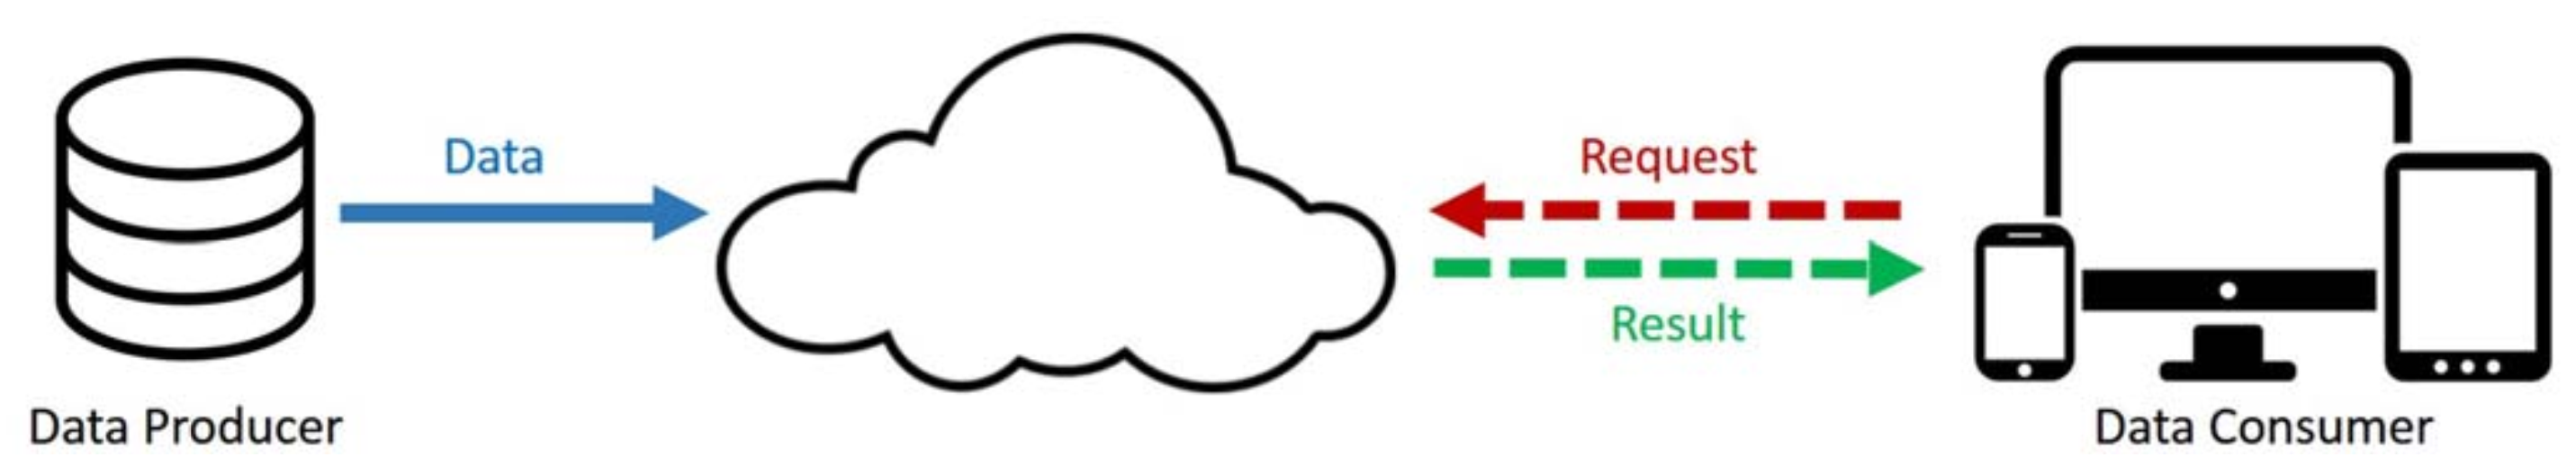
\includegraphics[width=10cm]{graphics/chapter_2/cloud_paradigm}}
            \caption{الگوی پردازش ابری \cite{shi2016edge}}
            \label{fig:chapter_2:cloud_paradigm}
          \end{figure}

        \item [تغییر از مصرف کننده داده به تولید کننده داده]
          در الگوی پردازش ابری، دستگاه‌های انتهایی در لبه شبکه معمولا نقش مصرف کننده داده را دارند.
          به عنوان نمونه می‌توان تماشای یک ویدیو را مثال زد.
          با این حال امروزه مردم در حال تولید داده توسط دستگاه‌هایشان هستند.
          برای مثال امروزه بسیار عادی است که افراد عکس‌ها و ویدیو‌هایی که توسط خودشان ضبط شده است را در سرویس‌های اینترنتی مختلف به اشتراک بگذارند.
          در \cite{2019domo} اشاره شده است که در هر دقیقه در \lr{twitter} ۵۱۱۲۰۰ توییت جدید ارسال می‌شود و در \lr{instagram} ۵۵۱۴۰ عکس جدید بارگذاری می‌شود.
          باید توجه داشت که این تصاویر و ویدیوها می‌توانند حجم زیادی داشته باشند و پهنای باند زیادی را برای بارگذاری استفاده کنند.
          در این موارد ویدیو‌ها باید ابتدا حجمشان در لبه شبکه کاهش پیدا کند تا به وضوح تصویر\LTRfootnote{resolution} مناسب برای بارگذاری در شبکه برسند.
          به عنوان نمونه‌ی دیگر می‌توان دستگاه‌های مربوط به سلامت را مثال زد.
          داده‌های جمع‌آوری شده توسط این دستگاه‌ها معمولا خصوصی است و پردازش این داده‌ها در لبه شبکه به جای ارسال داده‌ها برای پردازش به ابر به حفظ حریم خصوصی افراد کمک می‌کند.

      \end{description}
    
    \subsection{پردازش لبه چیست؟}
      پردازش لبه به همه تکنولوژی‌هایی اطلاق می‌شود که امکان انجام پردازش‌ها در لبه شبکه را فراهم می‌کنند.
      در اینجا منظور از لبه، همه منابع پردازشی و شبکه ای است که بین منبع داده‌ها (جایی که داده‌ها در آن جا تولید می‌شوند) و مراکز داده‌ی ابری قرار دارند.
      برای مثال یک دروازه‌ی شبکه در یک خانه هوشمند، می‌تواند یک منبع پردازشی لبه بین اشیاء و مرکز داده‌ی ابری باشد یا یک مرکز داده‌ی کوچک، می‌تواند یک منبع پردازشی لبه بین دستگاه‌های سیار و ابر در نظر گرفته شود.
      منطق در پردازش لبه این است که پردازش داده‌ها باید در همسایگی منبع داده‌ها انجام شود.
      با این منطق پردازش لبه و پردازش مه\cite{} دو مفهوم یکسان را خواهند داشت با این تفاوت که پردازش لبه تمرکزش سمت اشیاء است ولی پردازش مه تمرکزش سمت زیرساخت است.

      \begin{figure}[h]
        \centerline{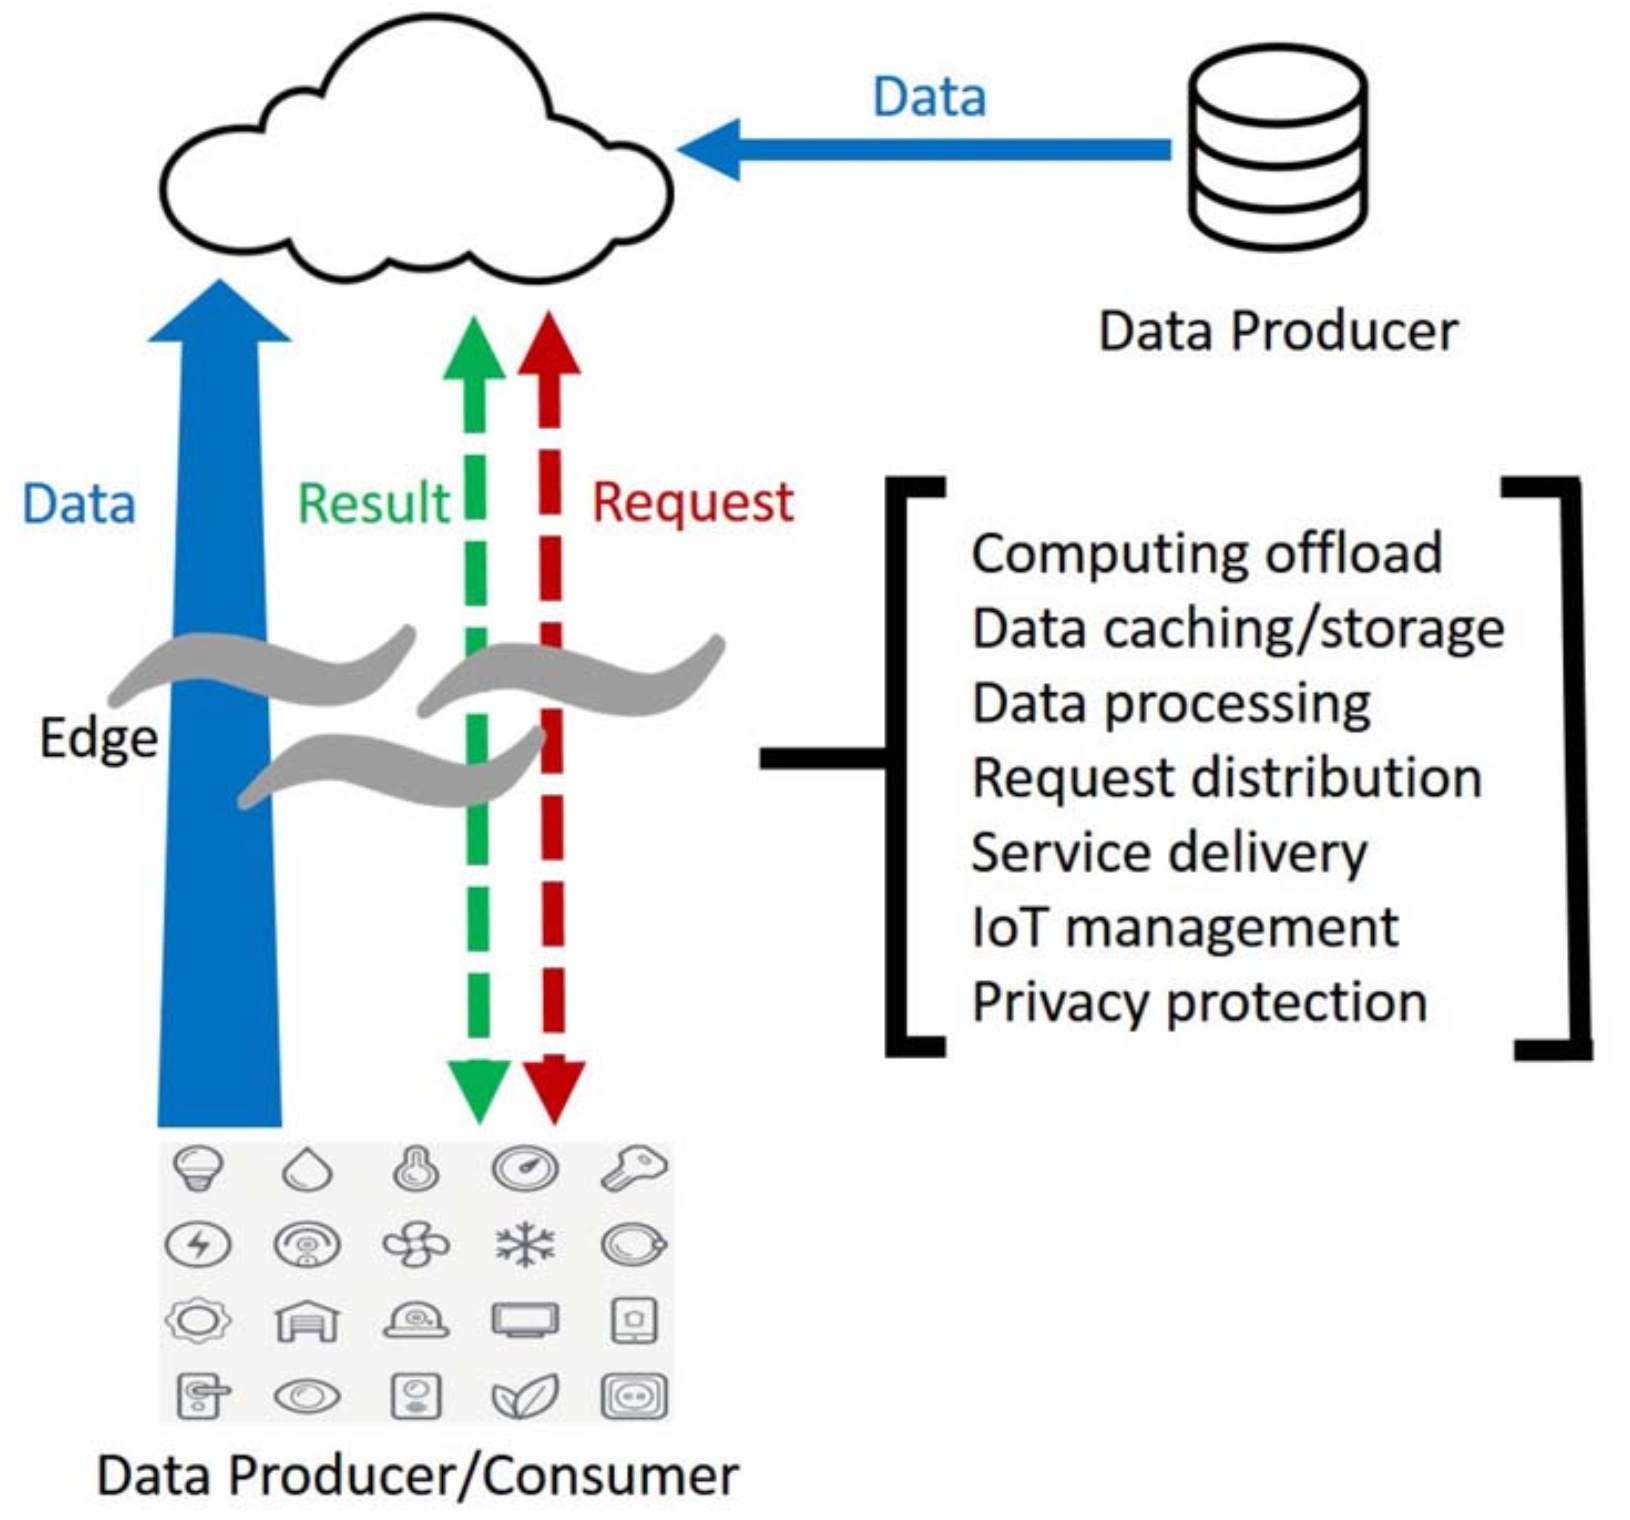
\includegraphics[width=10cm]{graphics/chapter_2/edge_paradigm}}
        \caption{الگوی پردازش لبه \cite{shi2016edge}}
        \label{fig:chapter_2:edge_paradigm}
      \end{figure}
      
      \cref{fig:chapter_2:edge_paradigm} جریان پردازش دو طرفه را در پردازش مه نشان می‌دهد.
      در الگو پردازش لبه، اشیاء نه تنها مصرف کننده داده بلکه تولید کننده‌ داده نیز هستند.
      در واقع در لبه، اشیاء نه تنها می‌توانند سرویس و محتوا از ابر درخواست نمایند بلکه می‌توانند وظایف پردازشی را هم انجام دهند.

    \subsection{مزایای پردازش لبه}
      همان طور که در بخش‌های قبل بیان شد، هدف از پردازش لبه قراردادن پردازش در مجاورت منبع تولید داده‌ها است.
      این کار مزایایی نسبت به روش‌های مبتنی بر پردازش ابری مرسوم دارد.
      در \cite{yi2015fog} برنامه‌ای برای تشخصی چهره ساخته شده است که با انتقال پردازش از ابر به لبه شبکه، زمان پاسخ برنامه از ۹۰۰ به ۱۶۰ میلی ثانیه کاهش پیدا کرده است.
      در \cite{ha2014towards} نویسندگان از واحدهای پردازشی ابری کوچک\LTRfootnote{Cloudlet} برای پردازش وظایف دستیار شناختی پوشیدنی\LTRfootnote{Wearable Cognetive Assitance} استفاده کرده اند و نتایج نشان می‌دهد که زمان پاسخ بین ۸۰ تا ۲۰۰ میلی ثانیه کاهش پیدا کرده است.
      روش ارائه شده در \cite{chun2011clonecloud} برای اجرای برنامه‌های تلفن همراه به کمک استفاده همزمان از پردازش ابری و پردازش لبه توانسته زمان اجرا و انرژی مصرفی را تا ۲۰ برابر کاهش دهد.

    \subsection{کاربرد پردازش لبه در شهر هوشمند}
      ویژگی‌های زیر باعث می‌شوند که پردازش لبه برای استفاده در شهر هوشمند مناسب باشد.
      \begin{enumerate}
        \item \textbf{حجم زیاد داده:}
          تخمین زده می‌شود که در سال ۲۰۱۹ میلادی یک شهر با جمعیت ۱ میلیون نفر، ۱۸۰ پتابایت داده در هر روز تولید می‌کند\cite{index2015forecast}.
          این داده‌ها توسط امنیت عمومی، سلامت، تجهیزات شهری و حمل و نقل تولید می‌شوند.
          ساختن مراکز داده‌ی متمرکز برای رسیدگی به همه‌ی این داده‌ها یک راهکار غیر واقعی است چرا که از این حجم از داده نیاز به قدرت پردازشی بسیار زیادی دارد.
          در این مورد پردازش لبه می‌تواند یک راه حل بهینه برای پردازش این حجم عظیم از داده‌ها باشد.

        \item \textbf{تاخیر کم:}
          برای کاربرد‌هایی که نیاز به تاخیر قابل پیشبینی و کم دارند مانند اورژانس سلامتی و امنیت عمومی، پردازش لبه یک الگوی مناسب است چرا که زمان انتقال داده‌ها را کاهش می‌دهد و ساختار شبکه را ساده‌تر می‌کند
        \item \textbf{آگاهی از مکان:}
          برای کاربرد‌های مبتنی بر موقعیت جغرافیایی مانند حمل و نقل و مدیریت تجهیزات شهری پردازش لبه به دلیل آگاهی از مکان بهتر از پردازش ابری عمل می‌کند.
      \end{enumerate}

    \subsection{مجازی سازی در پردازش لبه}
      در الگوی پردازش ابری برای به اشتراک گذاری منابع از روش‌های مبتنی بر مجازی سازی\LTRfootnote{Virtualization} استفاده می‌شود و فراهم کننده‌های سرویس‌های زیرساخت ابری\LTRfootnote{Cloud Infrastructure as a Service Providers} به کمک این روش‌ها می‌تواند منابع را به صورت سریع به اشتراک بگذارد \cite{pahl2015containers} و \cite{jain2016overview}.
      در پردازش ابری ماشین‌های مجازی \LTRfootnote{Virtual Machine} به عنوان اصلی ترین روش مجازی سازی مورد استفاده قرار می‌گیرند.
      کارآمدی ماشین‌های مجازی در طول زمان با بهبود روش‌های زمان بندی، بسته بندی و ارتقاء امنیت آن‌ها بیشتر شده‌است.
      هر ماشین مجازی سیستم فایل بندی\LTRfootnote{File System} خود را به عنوان یک فایل مجزا روی حافظه کامپیوتر میزبان ذخیر می‌کند و به عنوان یک پردازه\LTRfootnote{Proccess} بزرگ در کامپیوتر میزبان اجرا می‌شود.
      برای حفظ امنیت هر کدام از این ماشین‌های مجازی، آن‌ها به صورت ایزوله نسبت به هم اجرا می‌شوند.

      در این روش مجازی سازی، {\xecolor{red}هایپروایزر}\LTRfootnote{Hypervisor} وظیفه شبیه‌سازی در سطح سخت افزار را دارد.
      به همین دلیل ماشین‌های مجازی از کامپیوتر میزبان مستقل خواهند بود.
      این استقلال از کامپیوتر میزبان باعث می‌شود که ماشین‌های مجازی با سیستم عامل متفاوت از سیستم عامل میزبان قابل اجرا باشند\cite{morabito2015hypervisors}.
      با این حال این روش دارای محدودیت‌هایی هم هست.
      یکی از این محدودیت‌ها این است که تصویر سیستم عامل میزبان به صورت کامل برای تک تک ماشین‌های مجازی نیاز است که باعث مصرف زیاد حافظه ذخیره‌سازی تصادفی و دیسک می‌شود.
      از دیگر محدودیت‌های این روش این است که شبیه سازی دستگاه‌های سخت افزاری توسط {\xecolor{red}هایپروایزر}  باعث افزایش سربار پردازشی در کامپیوتر میزبان و کاهش بهره‌وری کلی می‌شود.
      علاوه بر این، این روش دارای زمان راه‌اندازی زیادی می‌باشد چراکه سیستم عامل تک تک ماشین‌های مجازی باید راه اندازی شود.
    از {\xecolor{red}هایپروایزر}های مشهور می‌توان \lr{KVM (Kernel Based Virtual Machine)}\cite{2019kvm}, \lr{VMware ESXi}\cite{2019esxi}, \lr{Xen}\cite{2019xen} و \lr{Microsoft Hyper-V}\cite{2019hyper} نام برد.
      \cref{fig:chapter_2:vm} ساختار معماری مبتنی بر {\xecolor{red}هایپروایزر} را نشان می‌دهد.

      \begin{figure}[]
        \centerline{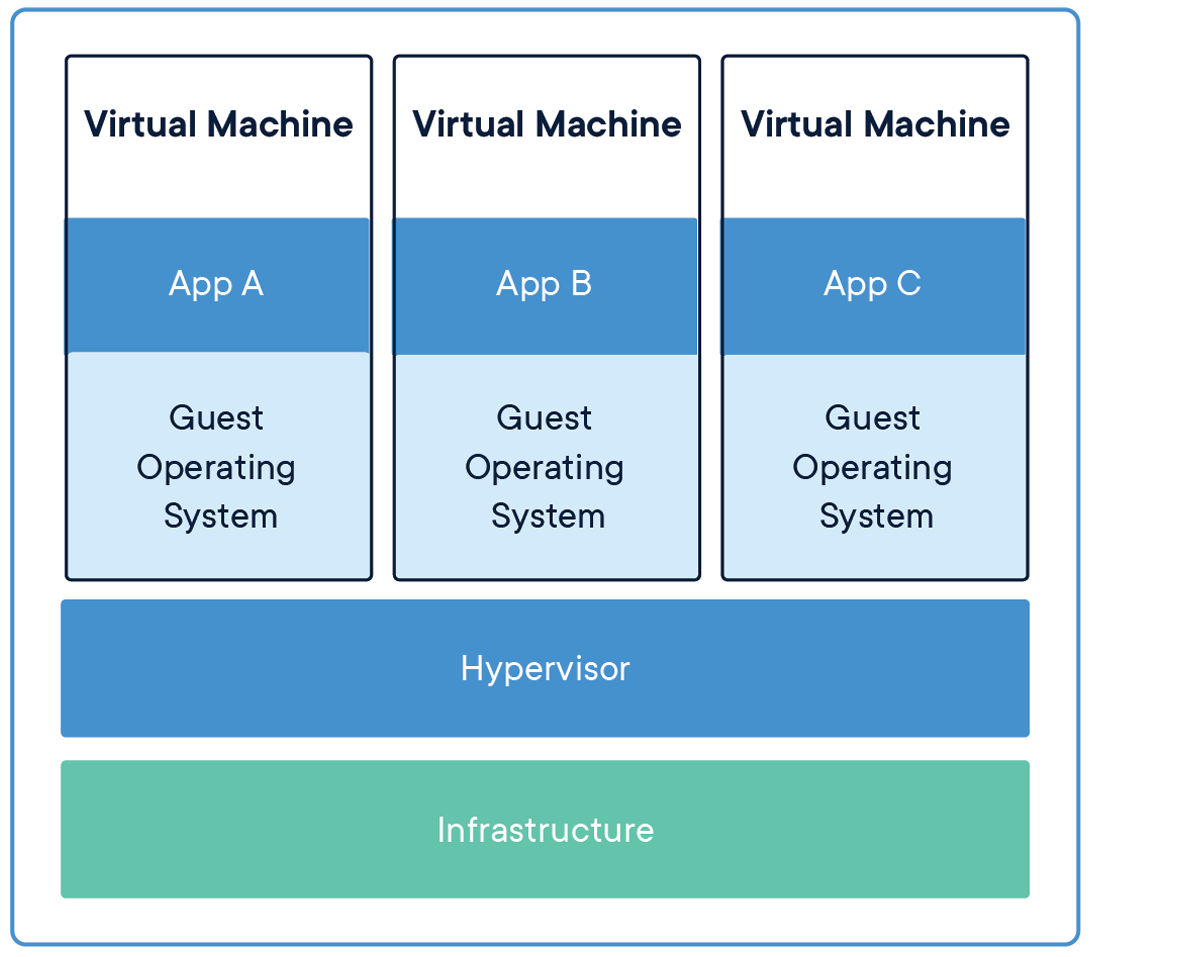
\includegraphics[width=10cm]{graphics/chapter_2/vm}}
        \caption{ساختار معماری مبتنی بر {\xecolor{red}هایپروایزر} \cite{2018are}}
        \label{fig:chapter_2:vm}
      \end{figure}

      روش‌های مجازی سازی مبتنی بر کانتینر\LTRfootnote{Container Based 
      Virtualization} مجازی سازی و ایزولاسیون را در سطی متفاوت از سطحی که روش‌های مبتنی بر {\xecolor{red}هایپروازر} انجام می‌دهند، دنبال می‌کنند.
      درواقع می‌توان آن‌ها را جایگزین سبکی برای روش‌های مجازی سازی مبتنی برای {\xecolor{red}هایپروازر} در نظر گرفت.
      در روش‌های مجازی سازی مبتنی بر {\xecolor{red}هایپروازر} یک سیستم عامل مجزا به طور کامل برای هر کدام از ماشین‌های مجازی اجرا می‌شود.
      در مقابل در روش‌های مبتنی بر کانتینر، ایزولایسون پردازه‌ها را در سطح سیستم عامل پیاده‌سازی می‌شود.
      برای این کار همه‌ی کانتینر‌ها بر روی یک سیستم عامل مشترک روی کامپیوتر میزبان اجرا می‌شوند و هر کانتینر می‌تواند شامل یک یا چند پردازه باشد.
      بنابراین سربار اجرای چندین سیستم عامل و راه‌انداز‌های سخت افزاری\LTRfootnote{Device Driver} و شبیه‌سازی سخت افزار‌های مختلف را از بین می‌برند.
      ساختار مجازی سازی مبتنی بر کانتیر در \cref{fig:chapter_2:container} نشان داده شده‌است.
            
      \begin{figure}[]
        \centerline{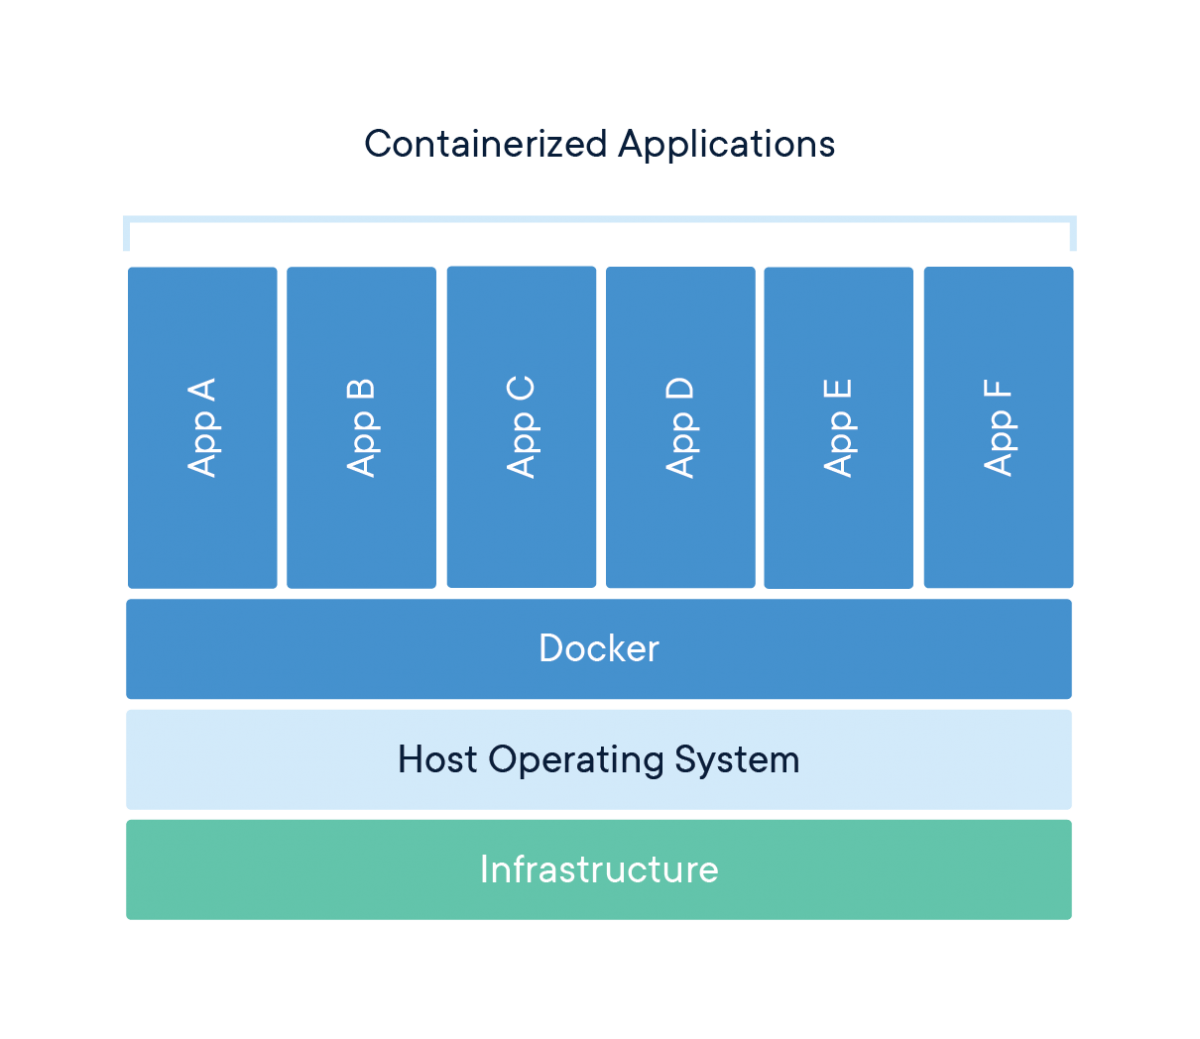
\includegraphics[width=10cm]{graphics/chapter_2/container}}
        \caption{ساختار مجازی سازی مبتنی بر کانتینر \cite{2018are}}
        \label{fig:chapter_2:container}
      \end{figure}
      
      مجازی سازی‌های مبتنی بر کانتینر در مقایسه با روش‌های مجازی سازی سخت افزاری مزایایی مانند سرعت ایجاد سریع‌تر دارند چرا که دیگر نیاز به شروع سیستم‌عامل جداگانه‌ای نیست.
      علاوه بر این سیستم‌های مبتنی بر کانتینر به دیلی حجم کم‌تر  تصویر‌ها\LTRfootnote{Image} و اجرا شدن روی هسته سیستم‌عامل\LTRfootnote{Operating System Kernel} مشترک می‌توانند تخصیص منابع بهتری داشته باشند \cite{morabito2015hypervisors}.

      با این حال استفاده از هسته‌ی سیستم عامل مشترک اشکالاتی در مقایسه با روش‌های مجازی‌سازی مبتنی بر {\xecolor{red}هایپروایزر} به همراه دارد.
      یکی از این اشکالات این است که کانتینر‌های سیستم عامل‌های مختلف قابل استفاده در سیستم عامل‌های دیگر نیستند.
      دیگر اشکال مجازی سازی‌های مبتنی بر کانتینر این است که ایزولاسیون در آن‌ها به خوبی روش‌های مجازی سازی مبتنی بر {\xecolor{red}هایپروایزر} نیست \cite{bui2015analysis} چرا که هسته سیستم عامل کامپیوتر میزبان در همه کانتینر‌ها مشترک است و این ممکن است برای امنیت در اجاره چندگانه\LTRfootnote{Multi-Tenant} مناسب نباشد.

      در ادامه به بررسی کانتینر‌ها در سیستم عامل لینوکس می‌پردازیم.
      در این سیستم عامل کانتینر‌ها به صورت عمده به وسیله‌ی گروه‌های کنترل\LTRfootnote{Control Groups (cgroups)}\cite{tejun2015Linux} و فضای نام‌ها\cite{2015Linux} پیاده‌سازی می‌شوند.

      گروه‌های کنترل در سال ۲۰۰۶ توسط مهندسان \lr{Google} توسعه داده‌شد و امکان مدریت منابع مانند، محدودیت استفاده از منابع یا اولویت پردازه‌ها را برای گروهی از پردازه‌ها مشخص می‌کنند.
      فضای‌نام‌ها هم یک دید محدود و اختصاصی برای منابع سیستم در هر کانتینر ایجاد می‌کند.
      مجموعه‌ای از پردازه‌ها می‌توانند در یک فضای نام قرار بگیرند و محدودیت‌های یکسانی را در استفاده از منابع برای آن‌ها تعریف کرد.
      هر کامپیوتر می‌تواند چندید فضای نام داشته باشد و برای هر کدام ویژگی منابع توسط هسته‌ی سیستم عامل اعمال می‌شود.
      اختصاص منابع به هر فضای نام می‌تواند به گونه‌ای باشد که استفاده از واحد پردازنده مرکزی\LTRfootnote{Central Processing Unit (CPU)}، حافظه‌ی با دسترسی تصادفی\LTRfootnote{Random Access Memory (RAM)} و سایر منابع را برای مجموعه‌ای از پردازه‌ها محدود کند.
      با اضافه شدن ایزولاسیون گروه‌های کنترل در هسته لینوکس امکان ایجاد فضای نام‌هایی که از فضای نام‌های دیگر مستقل باشند ممکن شد.
      چند مورد از مهم‌ترین ویژگی‌های ایزولاسیون در فضای نام‌ها را ادامه بررسی می‌کنیم:
      \begin{enumerate}
        \item \textbf{فضای نام‌های شناسه پردازه‌ها\LTRfootnote{Process Identifier(PID)}:} این ویژگی باعث می‌شود که پردازه‌های یک فضای نام، از پردازه‌های فضای نام‌های دیگر با خبر نباشند.
        \item \textbf{فضای‌نام‌های شبکه:} ایزولاسیون کنترل‌کننده‌های رابط‌های‌ شبکه\LTRfootnote{Network Interface Controller (NIC)}، جدول‌های مسیریابی و ابزار‌های سطح پایین شبکه را ممکن می‌سازد
        \item \textbf{فضای نام‌های دستگاه‌های سوار شده\LTRfootnote{Mount Namespace}:} از این ویژگی برای ایزولاسیون دستگاه‌های سوار شده استفاده می‌شود که باعث می‌شود بتوان روی مصرف فضای نام‌های مختلف از دیسک محدودیت گذاشت.
        \item \textbf{فضای‌نام‌های کاربران:} کاربران یک فضای نام را به همان فضای نام محدود می‌کند و مانع تداخل شناسه‌های کاربری\LTRfootnote{User Identifier (UID)} یکسان در فضای نام‌های مختلف می‌شود.
      \end{enumerate}
      به بیان ساده‌تر این ویژگی‌ها باعث می‌شوند که هر فضای نام به عنوان کامپیوتر پردازه‌هایی که در آن اجرا می‌شوند ظاهر شود.

      از راه حل‌های مبتنی بر کانتینر می‌توان \lr{Linux-VServer}\cite{2019vserver}، \lr{OpenVZ}\cite{2019openvz}، \lr{LXC}\cite{2019containers}، \lr{Docker}\cite{2019docker} و \lr{rtk}\cite{2019rtk} را نام برد.
      در بین این راه‌حل‌ها \lr{LXC} و \lr{Docker} از بقیه مشهورتر هستند.
      \lr{LXC} یک راه حل سطح پایین‌تر ارائه می‌دهد و زمان زیادی است که موجود است.
      در واقع LXC اولین پیاده‌سازی چیزی که ما امروزه به نام کانتینر می‌شناسیم است.
      \lr{LXC} با استفاده از مزایای گروه‌های کنترل و فضای نام‌ها یک محیط مجازی درست کند که پردازه‌ها به صورت جدا از هم اجرا شوند.
      می‌توان این گونه برداشت کرد که \lr{LXC} امکان وجود فضا‌های کاربری\LTRfootnote{User Space} ایزوله و جدا را روی یک کامپیوتر فراهم می‌کند.
      در مقابل \lr{Docker} در سال ۲۰۰۹ معرفی شد و یک راه حل سطح بالاتر ارائه می‌دهد.
      \lr{Docker} با ترکیب کردن کانتینر‌های لینوکس با یک سیستم فایل‌بندی لایه‌لایه و ارائه ابزار‌هایی برای ساخت و بسته‌بندی برنامه‌های کاربردی به صورت تصویر کانتینر‌ها توانست محبوبیت زیادی کسب کند.
      نخستین نسخه‌های \lr{Docker} به صورت مستقیم از \lr{LXC} استفاده می‌کردند.
      در حال خاضر \lr{Docker} محبوب‌ترین تکنولوژی کانتینر می‌باشد به طوری که بیشتر افراد وقتی از تکنولوژی کانتینر نام برده می‌شود، فقط \lr{Docker} را در نظر می‌گیرند.
      با وجود تکنولوژی‌های مختلف کانتینر که در بالا اشاره شد، \lr{Docker} به عنوان یک استاندارد صنعتی برای کانتینر‌ها پذیرفته شده‌است.
      با این وجود داکر بر روی گروه‌های کنترل و فضای‌نام‌های هسته لینوکس بنا شده‌است.

      کانتینر‌های \lr{Docker} از چندین لایه از تصویر‌ها ساخته شده‌اند.
      این تصویر‌ها شامل فایل‌هایی دودویی هستند که باهم در یک بسته‌بندی قرار داده‌ شده‌اند.
      ایمیج پایه سیستم عامل کانتینر را نگهداری می‌کند که می‌تواند متفاوت با سیستم عامل کامپیوتر باشد.
      سیستم عامل کانتینر، یک سیستم عامل کامل مانند سیستم عامل کامپیوتر میزبان نیست.
      تفاوت این است که تصویر تنها سیستم فایل بندی و فایل‌های دو دویی سیستم عامل را دارد ولی سیستم عامل کامپیوتر میزبان سیستم فایل بندی، فایل‌های دو دویی و هسته سیستم عامل را دارا می‌باشد.
      روی تصویر پایه، چندین تصویر قرار می‌گیرد که هر کدام بخشی از کانتینر را می‌سازند.
      در واقع هر تغییری روی فایل‌های تصویر‌های قبلی باعث ایجاد یک لایه جدید می‌شود.
      مزیت این روش این است که باعث کاهش فضای لازم برای نگهداری تصویر کانتینر‌ها می‌شود.
      برای مثال دو کانتینر را با لایه‌های تصویر آ، ب و ث برای کانتینر اول و آ، ب و ت برای کانتینر دوم در نظر بگیرید.
      با این روش نگهداری، لایه‌های تصویر آ و ب تنها یکبار ذخیره می‌گردند ولی اگر تصویر‌ها یکپارچه بودند برای هرکانتینر باید فضا اشغال می‌کردند.

      \begin{figure}[]
        \centerline{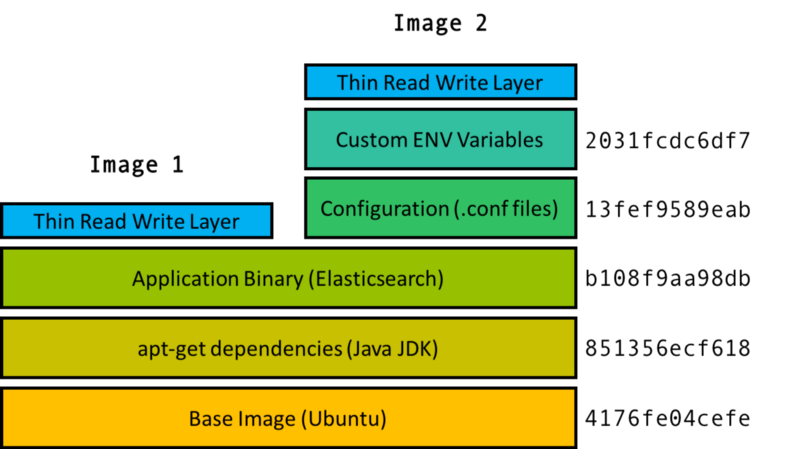
\includegraphics[width=10cm]{graphics/chapter_2/docker_image}}
        \caption{ساختار تصویر کانتینر‌ها در \lr{Docker} \cite{2019demystifying}}
        \label{fig:chapter_2:docker_image}
      \end{figure}

      در \lr{Docker} از نتیجه تابع در هم‌ساز\LTRfootnote{Hash} \lr{SHA-256} روی محتوای هر لایه به عنوان شناسه‌ی آن لایه‌ی تصویر استفاده می‌شود و هر لایه شناسه لایه‌های پایینی خود را نگهداری می‌کند و کانتینر‌ها با شناسه بالاترین تصویرشان متمایز می‌شوند.
      \cref{fig:chapter_2:docker_image}، ساختار تصویر دو کانتینر را نشان می‌دهد.
      همان طور که مشخص است این دو تصویر دارای سه لایه مشترک هستند و تصویر ۲ دارای دو لایه اضافی نیز هست.
      هنگامی که کانتینر اجرا می‌شود، \lr{Docker} ابتدا همه‌ی لایه‌های تصویر‌ها را بارگیری می‌کند.
      سپس گروه کنترل و نام‌دامنه‌های مربوط به کانتینر جدید را ایجاد می‌کند و از تصویر برای ایجاد محیط مجازی استفاده می‌کند به طوری که برای پردازه‌هایی که در آن کانتینر اجرا می‌شوند، انگار که فقط فایل‌های تصویر روی کامپیوتر قرار دارند.
      در انتها پردازه اصلی کانتینر را اجرا می‌کند.

      در \cite{ismail2015evaluation} نویسندگان \lr{Docker} را به عنوان تکنولوژی که امکان استفاده از پردازش لبه را فراهم می‌کند بررسی کرده‌اند.
      نویسندگان \lr{Docker} را در زمینه‌ی استقرار و پایان دادن سرویس‌ها، مدریت منابع و سرویس‌ها، تحمل خطا و ذخیره‌سازی مورد بررسی قرار دادند و نتیجه گرفتند که \lr{Docker} به عنوان یک راه حل مناسب برای استفاده در پردازش لبه قابل استفاده است.
      در \cite{viswanath2016system} و \cite{morabito2016enabling} از تکنولوژی‌های مجازی‌سازی سبک برای طراحی دروازه‌های\LTRfootnote{Gateway} اینترنت اشیاء استفاده شده‌است.
      در \cite{viswanath2016system} از یک نرم‌افزار مجازی سازی برای استقرار انبوه سرویس‌ها در لبه شبکه استفاده کرده‌اند.
      نکته قابل توجه در تحلیل آن‌ها، امکان اثر متقابل بین حسگر‌های اینترنت اشیاء و دروازه‌‌ها می‌باشد.
      تحلیل آن‌ها نشان می‌دهد که تخصیص پویای سرویس‌ها با استفاده از کانتینر‌ها مزایایی از بعد کارایی در دروازه‌ها دارد.
      در \cite{morabito2016enabling} یک طراحی برای دروازه‌های اینرنت اشیاء ارائه شده‌است که می‌تواند به صورت بهینه در لبه شبکه استفاده شود.
      بررسی‌های انجام‌شده در این مقاله کارآمدی و انعطاف پذیری استفاده از \lr{Docker} را برای استفاده در یک سکوی‌ اینترنت اشیاء که سرویس‌های مجازی مختلفی مانند مدریت دستگاه‌ها، پشتیبانی از شبکه‌های مبتنی بر نرم‌افزار\LTRfootnote{Software Defined Network (SDN)} و امکان مدریت و ساماندهی داده‌ها را ارائه دهد، نشان می‌دهد.
      در \cite{novo2015capillary} از \lr{Docker} برای بسته‌بندی، استقرار و اجرای نرم‌افزار‌ها در ابر و دستگاه‌های با منابع محدود مانند دروازه‌های خاصی استفاده شده‌است.
      هدف این دروازه‌ها فراهم کردن اتصال شبکه‌های با برد کوتاه با شبکه‌های سلولی و فراهم کردن اجزاء نرم‌افزار‌های مختلف برای مدریت دستگاه‌ها و پردازش‌های ابری توزیع‌شده می‌باشد.
      در \cite{celesti2016exploring} مجازی سازی مبتنی بر کانتینر و کامپیوتر‌های تک بردی\LTRfootnote{Single Board Computer (SBC)} به عنوان تکنولوژی‌هایی که امکان فراهم سازی سرویس‌های اینترنت اشیاء ابری را مهیّا می‌کنند، شناخته شده‌اند.
      مقاله \cite{krylovskiy2015internet} به شناسایی و بررسی نیازمندی‌های طراحی دروازه‌اینترنت اشیاء پرداخته است.
      نویسندگان کانتینر‌های \lr{Docker} را به عنوان تکنولوژی مناسب که این نیازمندی‌ها را برطرف می‌کند در نظر گرفتند.
      در این مطالعه، برای برآورد سربار لایه مجازی سازی از چند معیار ترکیبی و کاربردی استفاده شده‌است.
      با این حال، در این مطالعه، کارایی فقط برای برد \lr{Raspberry Pi} انجام شده و بررسی جامع مصرف توان و بهره‌وری انرژی در آن وجود ندارد.